\subsection{Obstacles}
Let us look at some of the obstacles we faced when creating tests. Some of these obstacles are specific to our grains, while other problems are more general. We will start by looking at the obstacles that are specific to the Orleans and Moq frameworks.
\subsubsection{GrainFactory} \label{GrainFactorySection}
In our grains we make use of GrainFactory to get the various grains in our adventure game for us. The way GrainFactory.GetGrain functions is that it looks through our silo, given a specified input id, and returns the grain, such that we can interact with it and call its functions. However, if we specify an id and our silo does not contain a grain corresponding to this id, it will not ignore or discard our request, but it will create a new grain for us and continue as planned. \todo{as explained in section 1.4 (?) about virtual actors} This is a problem when it comes to testing. As we mentioned and explained in \autoref{MockingSection}, to perform unit testing on our grains, we mock the grains that it depends on and communicates with. 
\begin{figure}[h]
    \centering
    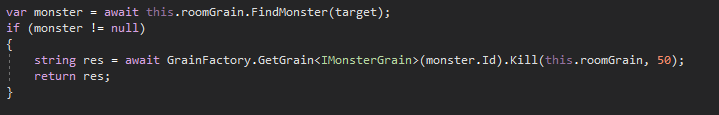
\includegraphics[width=\linewidth]{Materials/TestingTheory/FireballGrainFactory}
    \caption{Snippet of player's Fireball() function, showcasing the problem with GrainFactory. Even if our room was mocked and returned our mocked monster's id, GrainFactory would create a real monster based on this id, as it finds no monsters with this id.}
    \label{fireballGrainFactory}
\end{figure}
As we can see in \autoref{fireballGrainFactory}, our use of GrainFactory resides within some of the functions we wish to test in isolation. This means that if we wish to test this function in isolation from the other grains, we would create a mocked version of the monster, such that no real grain interferes in our test. However, the way GrainFactory works, this is not possible right out of the box. In our case, our GrainFactory would simply create a new monster grain for us, ignoring our mocked monster meant for the test and thus breaking our isolation of grains in the tests. So how do we get around this? We mock GrainFactory. \\
\\
As we went over in \autoref{MockingVsSection}, mocking a class means our mock is an inherited class that uses the base implementations. To override a function in an inherited class, the function must be of type virtual or abstract. Since the original GrainFactory contains neither of those modifiers, we will have to override the function in our grains. This means that in each of our grains we implement a 'public new virtual IGrainFactory GrainFactory' that fetches the base GrainFactory. By doing this, we can mock the grains' GrainFactory properties such that when GrainFactory is called doing a test, we return a specified mock instead of a new grain and we have thus enabled us to sidestep GrainFactory and keep our tests isolated. The downside to this is, of course, that our way of sidestepping this obstacle is by writing code in the grains that have no other use than in testing. In other words, this way of overcoming the obstacle included making test specific code, which is a bad practice\todo{cite. Only know the slides stating it}. \\
However, GrainFactory is our way of communication between grains and thus used in a lot of the functions across the grains. Because of this, we deemed it a necessary implementation, as exclusion of this mock would greatly decrease our possible tests, by making a range of functions across the grains unavailable for testing due to inclusion of GrainFactory.
\subsubsection{GetPrimaryKey}
In the player's TakeDamage() function we make use of the room's GetPrimaryKey to ensure that we are in the same room where we took damage. If we are not in the same room, we have dodged the attack and should not take any damage \todo{Mention distributed necessity for this?}. The GetPrimaryKey fetches the id of the specified grain. \\
This created some problems in testing however. GetPrimaryKey cannot be used by default in mocking of classes, meaning the comparison of GetPrimaryKey in TakeDamage() would fail and thus we could not test damage taken for the player. \\
Our initial idea here was to take the same route as with GrainFactory, that is mocking GetPrimaryKey, giving it some arbitrary value such that it would always pass the comparison and we could test damage taken in isolation. Apparently this is not possible, as GetPrimaryKey is non-overridable and inaccessible. This means that we would not be able to override it in the same way as GrainFactory and the mocking framework did not support use of GetPrimaryKey \todo{cite. Describe error, don't think you can find citation}. We thought of other ways to do the comparison of room id's, for instance with a public function that would return room's id from RoomInfo. We ultimately decided against this, because this would be too much alteration of code for the sole purpose of testing, which again is bad practice and should be avoided. The reason we decided against this, and not with GrainFactory, is due to the fact that the GetPrimaryKey comparison is only used in the case of TakeDamage, hence it is not vital for a lot of the tests. \\
With no apparent way around this issue, it means that currently the tests that use the TestDamage function in unit tests will fail. Fortunately, this only makes two tests fail, TakeDamageTest() and RoarTest(). Since we do not use mocking during integration testing, we do not face the issue of GetPrimaryKey in these cases, meaning that TakeDamage can be used in integration testing without this error. 
\subsubsection{Room Tests and Weather}
The way room and the different weather combination works is as follows. A room will have a combinated pool of weather to choose from. When a player enters a room, the room will then apply one of these weathers from the pool at random.\todo{Har vi forklaret room - weather connection før? I AdventureGame section} This way, a player will be affected by a random weather effect whenever entering a room, even if the player exit and enters the same rooms. Two of these weather effects affects the player directly, by either dealing damage to or healing the player upon entering the room. This proved difficult to control during testing. \\
\begin{figure}[h]
    \centering
    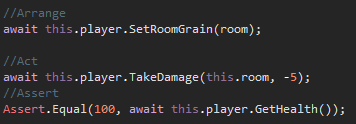
\includegraphics[width=0.5\linewidth]{Materials/TestingDiscussion/HailingWeatherDamageTest}
    \caption{An example of a player damage test that takes the weather into account. In this instance, because of the weather, we start with 95 health due to losing 5 by entering the room. What if the combinated game's seed chose the healing weather instead? Then the asserted health should be 115 and 105 if the weather did not affect the player.}
    \label{HailingWeatherDamageTest}
\end{figure}
During unit tests we use a mockup of the room interface, which means that the problem does not appear until the integration tests. What we did in the integration tests to keep the weather was to use a predetermined seed in our random number generator, giving us the same weather in all the tests. This was not sufficient though, as this weather, that dealt 5 damage to the player, may or may not be in the pool in a given variation of the game. So, even with a predetermined seed, we will not be able to determine which weather is used for the testing. This means that all tests that uses or asserts the players health when taking damage may be skewed. For instance, as we initially tested with all weathers active, we always had the damage dealing weather, so all our tests take into account that we start off with 95 health versus the original 100 start health. We can see an example of a test taking the weather into account in \autoref{HailingWeatherDamageTest}. Let us say that we combinated a variation without this weather, such that no damage was dealt to the player. These tests would then fail. Essentially we have three types of weather, one that does not affect the player, one that deals damage and one that heals. How can we ensure we keep the weather consistent or separated from the tests that use room, without knowing what our pool of weather is going to be? \todo{Solution eller non-solution}
\subsubsection{Newline Inconsistency}
It should also shortly be mentioned a minor problem we had, that we discarded as an unsolvable bug. Apparently, newline varies from operating system to operating system, meaning that a test could expect a "first line \textbackslash n second line", but the actual value is "first line \textbackslash r\textbackslash n second line". This mean that some of the tests may fail even though they are virtually the same except for the inconsistency of newline. We deemed this problem or bug unimportant as it has nothing to do with Orleans or the CLS and thus it has been ignored.

%Funktioner vi ikke kunne teste?